\scanpage{49}
\margin{15}
topologiques paracompacts, à un théorème d'isomorphisme pour les \deleted{préfa} préfaisceaux [T.F Chap. II, § 5, Th. 10.2] comme on s'en convainc facilement en examinant le cas des préfaisceaux constants.

Cependant, la notion introduite ici coincide avec celle de [T.F.] dans le cas particulier des préfaisceau abéliens $P$ tel que $P(\varnothing)=0$, condition vérifiée par exemple par les préfaisceaux $\mathcal H^q(F)$ \deleted{\unsure{qui}} qui s'introduisent dans la suite spectrale de Leray.
\margin{\figure{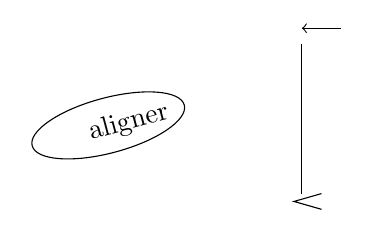
\begin{tikzpicture}[x=1cm,y=1cm]
\node[rotate=15] at (0,1) {aligner};\draw[rotate=15] (0,1) ellipse (1 and .35);
\draw[->] (2.7,2.2)--(2.2,2.2);\draw (2.2,2)--(2.2,.1);\draw (2.45,-.1)--(2.1,0)--(2.45,.1);
\end{tikzpicture}}}

Enfin soit $\deleted{\unsure{\lambda}}\ a:\widehat C_A\longrightarrow\widetilde C_A$ le foncteur faisceau associé. Le foncteur $a$ est exact. Il est adjoint à gauche au foncteur $\mathcal H^0$. Le morphisme d'adjonction :
\[a\mathcal H^0\longrightarrow\operatorname{id}_{\widetilde C_A}\qquad(21)\]
est un isomorphisme (2.3.14.II).

La formule d'adjonction fournit pour tout préfaisceau d'ensembles $S$ sur $C$ et tout faisceau de $A$-modules $F$ un isomorphisme :
\inserted{$F(aS)\xrightarrow{\sim}\mathcal H^0(F)(S)$ i.e.:}
\margin{$\unsure{\rho}\quad\unsure{\rho}$}
\[
\deleted{H^0(\unsure{C|\widetilde C}/aS,F)\unsure{\longrightarrow}H^0(\widehat C/S,F)=H^0(\widehat C/S,}
\]
\[H^0(\widetilde C/aS,F)\xrightarrow{\sim}H^0(\widehat C/S,\mathcal H^0(F))\qquad(22)\]

De plus si $G$ est un préfaisceau de $A$-modules tel que le faisceau associé soit nul, on a ((2.3.12.II) et (2.3.14.II)) :
\[\check{\mathcal H}^{0}(G)=0\qquad(23)\]
\margin{\figure{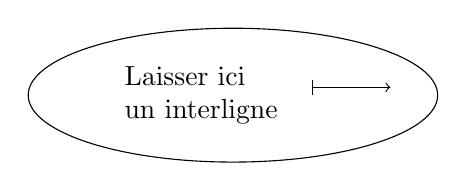
\begin{tikzpicture}[x=1cm,y=1cm]
\node[align=left,anchor=west] at (-1.5,0) {Laisser ici\\un interligne};
\draw (0,0) ellipse (2.6 and .85);\draw[|->] (1,.1)--(2,.1);
\end{tikzpicture}}}

Nous allons maintenant énoncer les propositions liant la cohomologie de Čech à la cohomologie des faisceaux.

\uline{Proposition 2.2} : Le foncteur $\mathcal H^0$ transforme les faisceaux injectifs en préfaisceaux injectifs. Soit $F$ un faisceau de $A$-modules. Les faisceaux associés aux préfaisceaux $\mathcal H^q(F)$ $(q>0)$ sont nuls.
\margin{\figure{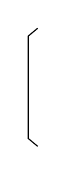
\begin{tikzpicture}\draw (.12,1.5)--(0,1.4)--(0,.1)--(.12,0);\end{tikzpicture}}}

\uline{Preuve} : Le foncteur faisceau associé, adjoint à gauche du foncteur $\mathcal H^0$ est exact; d'où la première assertion (0.2). Le foncteur $a\mathcal H^0$ est isomorphe au foncteur identique (formule (21)) d'où la deuxième assertion.

\uline{Proposition 2.3} : Soit $S$ un préfaisceau d'ensembles sur $C$.

Il existe une suite spectrale fonctoriel\inserted{le} en $S$ et $F$ :
\[\deleted{H^{p+q}(C/\unsure{U},F)}\]
\[H^{p+q}(\widetilde C/aS,F)\Longleftarrow H^p(\widehat C/S,\mathcal H^q(\unsure{F|E}))\]
\margin{\figure{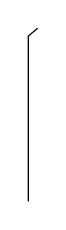
\begin{tikzpicture}\draw (.12,2.2)--(0,2.1)--(0,0);\end{tikzpicture}}}
\margin{48}
